\documentclass[11pt]{article}

\usepackage[letterpaper,margin=1in]{geometry}
\usepackage[T1]{fontenc}
\usepackage[utf8]{inputenc}
\usepackage{lmodern}
\usepackage{microtype}
\usepackage{amsmath,amssymb,mathtools,bm}
\usepackage{xcolor,slashed,needspace}
\usepackage{enumitem}
\usepackage{hyperref}
\usepackage[most]{tcolorbox}
\usepackage{fancyhdr}
\usepackage{parskip}

\definecolor{qftblue}{HTML}{245A8D}
\definecolor{qftgray}{HTML}{F4F6F8}
\hypersetup{
  colorlinks=true,
  linkcolor=qftblue,
  urlcolor=qftblue,
  pdftitle={PHYS 662 Homework 5 Solutions},
  pdfauthor={Nima Lashkari}
}

\pagestyle{fancy}
\fancyhf{}
\lhead{PHYS 662: Quantum Field Theory I}
\rhead{Homework 5 Solutions}
\cfoot{\thepage}
\setlength{\headheight}{14pt}

\setlist[enumerate]{leftmargin=2.2em,itemsep=0.55em,topsep=0.5em}
\newlist{parts}{enumerate}{1}
\setlist[parts]{label=\textbf{(\alph*)},leftmargin=2.3em,itemsep=0.65em}

\newcommand{\dd}{\mathrm{d}}
\newcommand{\ii}{\mathrm{i}}
\newcommand{\R}{\mathbb{R}}
\newcommand{\C}{\mathbb{C}}
\newcommand{\Z}{\mathbb{Z}}
\newcommand{\Lag}{\mathcal L}
\newcommand{\tr}{\operatorname{tr}}
\newcommand{\Ad}{\operatorname{Ad}}

\newtcolorbox{conventionbox}[1][]{
  enhanced,breakable,
  colback=qftgray,colframe=qftblue,
  boxrule=0.8pt,arc=1.5mm,
  title={#1},fonttitle=\bfseries,coltitle=white
}
\newcommand{\problem}[2]{%
  \Needspace{10\baselineskip}
  \section*{\color{qftblue}Problem #1: #2}
  \addcontentsline{toc}{section}{Problem #1: #2}
}
\newcommand{\lectureconnection}[1]{%
  {\small\textit{Lecture connection: #1.}\par}\medskip
}


\newcommand{\diag}{\operatorname{diag}}
\newcommand{\SO}{\mathrm{SO}}
\newcommand{\SU}{\mathrm{SU}}
\newcommand{\SL}{\mathrm{SL}}
\newcommand{\ISO}{\mathrm{ISO}}
\newcommand{\ddPi}{\dd\Pi}
\newcommand{\vac}{\lvert0\rangle}
\newcommand{\vbra}{\langle0\rvert}
\newcommand{\Dc}{\mathcal C}
\newcommand{\one}{\mathbf1}

\usepackage{booktabs,tikz}
\newcommand{\hc}{\mathrm{h.c.}}
\newcommand{\partsol}[2]{\par\Needspace{4\baselineskip}\medskip\noindent\textbf{(#1) #2.}\quad}

\begin{document}
\begin{center}
{\scshape\Large PHYS 662 --- Quantum Field Theory I\par}
\medskip
{\Huge\bfseries\color{qftblue} Homework 5 Solutions\par}
\medskip
{\large Lectures 15--16 \quad Fall 2026\par}
\end{center}
\begin{conventionbox}[Conventions and scope]
These solutions cover every part of all eight problems, including the two
added problems. The lecture references use the merged two-lecture sequence.
Use \(\eta=(+---)\), \(p\cdot x=E_pt-\bm p\cdot\bm x\), and
\(d\Pi_p=d^dp/[(2\pi)^d2E_p]\). Except in the explicitly general-dimensional
parts, \(d=3\). Mass is positive unless a limit is requested.
\[
 D^+(z)=\langle0|\phi(x)\phi(y)|0\rangle,\qquad
 \mathcal K(z)=D^+(z)-D^+(-z),\qquad L=\Box+m^2,
\]
\[
 G_R=i\theta(t)\mathcal K,\quad G_A=-i\theta(-t)\mathcal K,\quad
 D_F=\langle0|T\phi(x)\phi(y)|0\rangle,\quad G_F=iD_F.
\]
Spinor matrices match Lectures 13--16; \(\bar\Psi=\Psi^\dagger\gamma^0\),
\(S^{\mu\nu}=i[\gamma^\mu,\gamma^\nu]/4\), and
\(\gamma_*=-i\gamma^0\gamma^1\gamma^2\gamma^3\).
The step-function formulas and pole prescriptions are distributions.
\end{conventionbox}
\begingroup\small\tableofcontents\endgroup
\clearpage
\problem{1}{Retarded and advanced Green functions}
\partsol{a}{Homogeneous equation and initial data}
Each plane wave has \(p^2=m^2\), so \(L\mathcal K=0\). At \(t=0\),
the two terms cancel under \(\bm p\to-\bm p\). Differentiating first gives
\[
 \partial_t\mathcal K(0,\bm r)
 =-\frac i2\int\frac{d^3p}{(2\pi)^3}
       (e^{i\bm p\cdot\bm r}+e^{-i\bm p\cdot\bm r})
 =-i\delta^{(3)}(\bm r).
\]
This agrees with \([\dot\phi(0,\bm x),\phi(0,\bm y)]
=[\pi(0,\bm x),\phi(0,\bm y)]=-i\delta^{(3)}(\bm x-\bm y)\).

\partsol{b}{The distributional source}
For a smooth-in-time distribution f with \(f(0)=0\),
\(\delta'f=-f'(0)\delta\). Thus
\[
 L(\theta f)=\theta Lf+2\delta f'+\delta'f
            =\theta Lf+\delta f'(0),\quad
 L(\theta(-t)f)=\theta(-t)Lf-\delta f'(0).
\]
Multiplying by i and \(-i\), respectively, proves
\(LG_R=LG_A=\delta(t)\delta^{(3)}(\bm r)\).
Giving the two step functions the same prefactor would instead give
opposite sources. The naive factor two from \(2\delta f'\) is reduced by
\(\delta'f\); dropping that term is incorrect.

\partsol{c}{Spatial Fourier transform}
For each spatial momentum the homogeneous equation is
\((\partial_t^2+E_p^2)\widetilde{\mathcal K}=0\), with initial values
0 and \(-i\). Hence
\[
 \widetilde{\mathcal K}(t,\bm p)=-i\frac{\sin(E_pt)}{E_p},\quad
 G_R(t,\bm p)=\theta(t)\frac{\sin(E_pt)}{E_p},\quad
 G_A(t,\bm p)=-\theta(-t)\frac{\sin(E_pt)}{E_p}.
\]
Both G functions have derivative jump +1 across zero; G itself is continuous.

\partsol{d}{Pole locations and residues}
Since L acts in Fourier space as \(-(p^0)^2+E_p^2\), its inverse is
\[
 \widetilde G_R(p)=-\frac1{(p^0+i0)^2-E_p^2},\qquad
 \widetilde G_A(p)=-\frac1{(p^0-i0)^2-E_p^2}.
\]
Both retarded poles are below the real axis, and both advanced poles
are above. The diagrams also include the Feynman prescription needed in
Problem 2; the vertical displacement is schematic.
\begin{center}
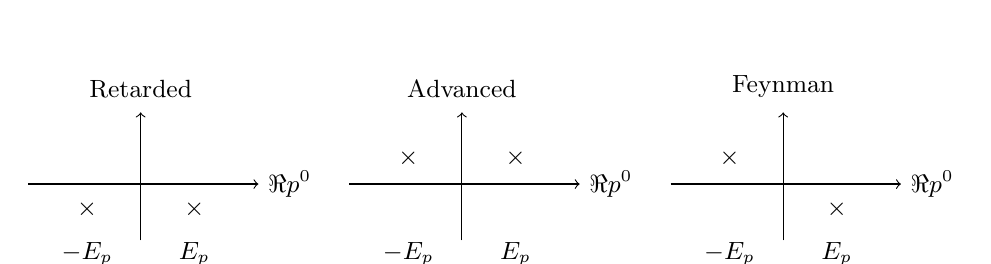
\begin{tikzpicture}[x=0.68cm,y=0.65cm,font=\small]
\foreach \shift/\title/\ym/\yp in {0/Retarded/-0.5/-0.5,6/Advanced/0.5/0.5,12/Feynman/0.5/-0.5}{
 \begin{scope}[xshift=\shift*0.68cm]
 \draw[->] (-2.1,0)--(2.2,0) node[right] {\(\Re p^0\)};
 \draw[->] (0,-1.1)--(0,1.4);
 \node[above] at (0,1.5) {\title};
 \node at (-1,\ym) {\(\times\)}; \node at (1,\yp) {\(\times\)};
 \node[below] at (-1,-0.95) {\(-E_p\)};\node[below] at (1,-0.95) {\(E_p\)};
 \end{scope}}
\end{tikzpicture}
\end{center}
For \(e^{-ip^0t}\), close below clockwise when \(t>0\), above
counterclockwise when \(t<0\). For the retarded case the sum of the
residues at \(\pm E_p-i0\) is
\((-e^{-iE_pt}+e^{iE_pt})/(2E_p)=i\sin(E_pt)/E_p\).
The clockwise factor \(-i\), including \(1/(2\pi)\), gives the positive
sine for \(t>0\). For \(t<0\) there are no enclosed poles.
The advanced contour has no poles for \(t>0\); for \(t<0\) its
counterclockwise factor \(+i\) gives \(-\sin(E_pt)/E_p\).

\partsol{e}{Source response}
The term \(+J\phi\) gives \(L\phi=J\). With a fixed incoming homogeneous
solution \(\phi_{\rm in}\), the solution with no incoming disturbance is
\[
 \phi(x)=\phi_{\rm in}(x)+\int d^4y\,G_R(x-y)J(y).
\]
The commutator vanishes at spacelike separation by Lorentz covariance
and the equal-time bracket; multiplication by \(\theta(x^0-y^0)\) then
restricts support to the future cone. The convolution is zero outside
the causal future of \(\operatorname{supp}J\). Using \(G_A\) instead fixes
no outgoing disturbance in the future and generally produces a response
before the source, rather than the retarded initial-value solution.

\partsol{f}{Why the equation is insufficient}
Since \(\theta(t)+\theta(-t)=1\) distributionally here,
\(G_R-G_A=i\mathcal K\). It is a nonzero homogeneous solution. Thus the
unit-source equation alone leaves freedom to add homogeneous solutions;
support or other boundary conditions select an inverse.

\problem{2}{The Feynman function as an inverse wave operator}
\partsol{a}{The equal-time jump}
The two pieces of \(D_F\) agree at \(t=0\), so D has no value jump.
Its derivative jump is
\[
 [\partial_tD_F]_{0^-}^{0^+}
 =\partial_t[D^+(t,\bm r)-D^+(-t,-\bm r)]_{t=0}
 =-i\delta^{(3)}(\bm r).
\]
Consequently \(LD_F=-i\delta^{(4)}\), and \(LG_F=\delta^{(4)}\) for
\(G_F=iD_F\). The source is fixed by the canonical algebra, not by the
name assigned to the propagator.

\partsol{b}{Feynman poles}
Fourier transforming the source equation gives
\((p^2-m^2)\widetilde D_F=i\). Time ordering chooses
\(p^0=E_p-i0\) and \(p^0=-E_p+i0\), as drawn in Problem 1.
For \(t>0\), the positive pole has residue
\(i e^{-iE_pt}/(2E_p)\), and clockwise closure gives
\(e^{-iE_pt}/(2E_p)\). For \(t<0\), the negative pole has residue
\(-i e^{iE_pt}/(2E_p)\); counterclockwise closure gives
\(e^{iE_pt}/(2E_p)\). Restoring the spatial Fourier transform gives
\[
 D_F(z)=\int\frac{d^4p}{(2\pi)^4}
       \frac{i e^{-ipz}}{p^2-m^2+i0}
       =\theta(t)D^+(z)+\theta(-t)D^+(-z).
\]
In the negative-time term change \(\bm p\to-\bm p\) to match the last form.

\partsol{c}{Boundary condition versus causal response}
The retarded poles both lie below, whereas Feynman puts one on each
side. Since both \(G_F\) and \(G_R\) have unit source,
\(L(G_F-G_R)=0\). Their difference need not be zero.
At spacelike separation \(D_F=D^+\) can be nonzero, so \(G_F\) is not
the retarded response kernel. Local influence depends on the commutator,
which vanishes there, rather than on the time-ordered vacuum correlation.

\partsol{d}{Fermionic time ordering}
In components, with \(t=x^0-y^0\),
\[
 (S_F)_{\alpha\beta}
 =\theta(t)\langle\Psi_\alpha(x)\bar\Psi_\beta(y)\rangle
 -\theta(-t)\langle\bar\Psi_\beta(y)\Psi_\alpha(x)\rangle.
\]
The exchange of the two odd fields gives the second minus sign. Mode
contraction and the two spin sums give
\[
 S_F(z)=\theta(t)\int d\Pi_p(\slashed p+m)e^{-ipz}
       -\theta(-t)\int d\Pi_p(\slashed p-m)e^{ipz}.
\]
Acting with \(i\slashed\partial+m\) on the two scalar pieces gives just
these numerators: \((\slashed p+m)\) and \((-\slashed p+m)\).
There is no extra step-function contact term in this first derivative,
because the scalar D has no value jump. Thus
\(S_F=(i\slashed\partial+m)D_F\).

\partsol{e}{The local Dirac source}
It follows that
\[
 S_F(z)=\int\frac{d^4p}{(2\pi)^4}
       \frac{i(\slashed p+m)e^{-ipz}}{p^2-m^2+i0},\qquad
 (i\slashed\partial-m)S_F
 =-(\Box+m^2)D_F\,I_4=i\delta^{(4)}I_4.
\]
Equivalently its first-order source is \(i\gamma^0\delta(t)\) times the
jump of S. With fermionic time ordering that jump is
\(\langle\{\Psi(0,\bm x),\bar\Psi(0,\bm y)\}\rangle
=\gamma^0\delta^3(\bm x-\bm y)\).
Omitting the exchange minus replaces this anticommutator by a
commutator whose mode numerator does not give the equal-time identity.
It therefore fails the local source equation.

\problem{3}{Massive two-point functions in arbitrary dimension}
\partsol{a}{Gaussian evaluation}
Insert the supplied Schwinger parameter at \(t=0\), retaining the factor
\(1/2\) in the invariant measure. The Gaussian momentum integral gives
\[
 D_d^+(0,r)=\frac1{2\sqrt\pi(4\pi)^{d/2}}
  \int_0^\infty d\alpha\,\alpha^{-(d+1)/2}
           e^{-m^2\alpha-r^2/(4\alpha)}.
\]
Set \(\nu=(d-1)/2\), \(a=m^2\), \(b=r^2/4\) in the supplied Bessel
integral. Simplifying the powers of 2 gives
\begin{equation}
 \boxed{D_d^+(0,r)=\frac{m^\nu}{(2\pi)^{\nu+1}r^\nu}K_\nu(mr),
        \qquad \nu=\frac{d-1}{2}.}
 \label{sol5:bessel}
\end{equation}
The dimension is \(2\nu=d-1=2[\phi]\); the Bessel argument is dimensionless.

\partsol{b}{Low-dimensional checks and coincidence}
The first three answers are
\[
 D_1^+=\frac{K_0(mr)}{2\pi},\qquad
 D_2^+=\frac{e^{-mr}}{4\pi r},\qquad
 D_3^+=\frac{mK_1(mr)}{4\pi^2r}.
\]
The middle one follows immediately from \(K_{1/2}\).
At coincidence the underlying momentum integral is ultraviolet divergent;
these expressions at \(r>0\) do not define pointwise field products at
\(r=0\). Their extension is a distribution, and coincident composite
operators require an additional prescription.

\partsol{c}{Large spacelike distance}
Using the supplied asymptotic formula yields
\[
 D_d^+(0,r)\sim
 \frac{m^{(d-2)/2}}{2(2\pi)^{d/2}r^{d/2}}e^{-mr}
 \left[1+O((mr)^{-1})\right].
\]
The exponential scale is the Compton wavelength \(m^{-1}\).
The power \(r^{-d/2}\) is part of the leading answer and cannot be
absorbed into a distance-independent coefficient.

\partsol{d}{Timelike boundary value and stationary phase}
The full positive-frequency boundary value is the expression in
\eqref{sol5:bessel} with
\(r\to\rho_\epsilon=\sqrt{r^2-(t-i\epsilon)^2}\), continued from positive
real \(\rho\). For \(t>0\) timelike, \(\rho\to+i\sqrt{t^2-r^2}\);
for \(t<0\), \(\rho\to-i\sqrt{t^2-r^2}\).
Changing the sign of \(i\epsilon\) interchanges these boundary values and
the frequency orientation; a function of \(z^2\) without that prescription
is incomplete. Independently, at \(\bm r=0\), \(mt\gg1\), \(t>0\),
\[
 E_p=m+\frac{\bm p^2}{2m}+\cdots,\qquad
 D_d^+(t,0)\sim\frac{e^{-imt}}{2m}
 \int\frac{d^dp}{(2\pi)^d}e^{-it\bm p^2/(2m)}
 =\frac{e^{-imt-i\pi d/4}}{2m}
       \left(\frac{m}{2\pi t}\right)^{d/2}.
\]
The Gaussian is defined with the same convergence prescription.
Corrections are of relative order \(1/(mt)\); negative times give the
complex conjugate. There is oscillation with a power envelope, not
spacelike exponential decay in \(|t|\).

\partsol{e}{Massless limit}
For \(d>1\), \(\nu>0\) and
\(K_\nu(z)\sim2^{\nu-1}\Gamma(\nu)z^{-\nu}\). Hence
\[
 D_d^+(0,r)\longrightarrow
 \frac{\Gamma((d-1)/2)}{4\pi^{(d+1)/2}r^{d-1}}.
\]
For \(d=1\), instead
\(D_1^+\sim-[\log(mr/2)+\gamma_E]/(2\pi)\).
Its \(-\log m\) term is an infrared-divergent additive constant. One must
specify an infrared scale/zero-mode prescription, or work with differences
or derivatives that remove the constant. It is not the \(d>1\) power law.

\problem{4}{The commutator, its light-cone terms, and locality}
\partsol{a}{General dimension and time orientation}
Interchanging z and \(-z\) swaps the two mass-shell integrals, proving
oddness. On-shell momenta give \(L\mathcal K_d=0\). For spacelike z a
proper orthochronous transformation brings it to \(t=0\), where
\(\bm p\to-\bm p\) cancels the two integrals. This proves spacelike
vanishing without assuming that the individual Wightman functions vanish.
For \(\tau=\sqrt{t^2-r^2}>0\) let
\(F_\nu(\rho)=m^\nu K_\nu(m\rho)/[(2\pi)^{\nu+1}\rho^\nu]\).
The timelike answer away from the cone is
\[
 \mathcal K_d(t,\bm r)=\operatorname{sgn}(t)
  \lim_{\epsilon\downarrow0}
 [F_\nu(\epsilon+i\tau)-F_\nu(\epsilon-i\tau)].
\]
This form retains the information lost by specifying only \(z^2=\tau^2\).

\partsol{b}{The cone and interior in three spatial dimensions}
Put \(\sigma=t^2-r^2\). The leading term of \(K_1(m\rho)\) gives
\(D^+\sim1/(4\pi^2\rho^2)
=-[4\pi^2(\sigma-i0\operatorname{sgn}t)]^{-1}\).
Using the stated boundary-value identity, its discontinuity is
\(-i\operatorname{sgn}(t)\delta(\sigma)/(2\pi)\).
For the interior, the Bessel connection formula
\(K_1(ix)=-\frac\pi2[J_1(x)-iY_1(x)]\), \(x>0\), gives
\[
 D^+(t,r)\big|_{t>0,\sigma>0}
 =\frac{m}{8\pi\sqrt\sigma}
     [Y_1(m\sqrt\sigma)+iJ_1(m\sqrt\sigma)].
\]
Subtract its conjugate and combine the cone term:
\begin{equation}
 \boxed{\mathcal K(t,r)=-i\operatorname{sgn}(t)
 \left[\frac{\delta(\sigma)}{2\pi}
 -\theta(\sigma)\frac{mJ_1(m\sqrt\sigma)}{4\pi\sqrt\sigma}\right].}
 \label{sol5:commdist}
\end{equation}
Thus \(A=1/(2\pi)\), \(B=-1/(4\pi)\). As a normalization check, smear
at small positive t with a smooth spatial test function f. The delta
term integrates to \(-it f(0)+O(t^3)\):
\(\int_0^\infty r^2dr\,\delta(t^2-r^2)=t/2\), and the angular factor
is \(4\pi\). Since \(mJ_1(m\sqrt\sigma)/\sqrt\sigma\to m^2/2\), the
interior contribution is \(O(t^3)\). Differentiating at zero therefore
gives exactly \(-if(0)\), the required initial derivative.

\partsol{c}{Massless propagation in different dimensions}
At fixed separation \(mJ_1(m\sqrt\sigma)/\sqrt\sigma=O(m^2)\), so in
3+1 dimensions only the cone term survives:
\[
 G_R^{(3)}(t,r)=\theta(t)\frac{\delta(t^2-r^2)}{2\pi}
              =\frac{\delta(t-r)}{4\pi r}\quad(r>0).
\]
In 1+1 dimensions, the solution of the massless wave equation with
initial displacement zero and initial velocity \(\delta(x)\) is, by
integrating the d'Alembert formula,
\[
 G_R^{(1)}(t,x)=\frac12\theta(t)\int_{x-t}^{x+t}\delta(y)\,dy
              =\frac12\theta(t-|x|).
\]
Its support fills the interior as well as the boundary. Propagation
only on the cone is not universal in dimension; a mass also produces
the interior tail in \eqref{sol5:commdist}.

\partsol{d}{The role of the second charge sector}
The independent oscillator families give
\[
 [\Phi(x),\Phi^\dagger(y)]
 =\int d\Pi_p(e^{-ipz}-e^{ipz})=\mathcal K(z),\qquad
 [\Phi(x),\Phi(y)]=0.
\]
The negative term is from \([b^\dagger,b]\), whose order is reversed.
It cancels the positive-frequency term at spacelike z. Dropping the
creation term leaves \([\Phi_+(x),\Phi_+^\dagger(y)]=D^+(z)\), which is
nonzero there. Positive excitation energies do not justify removing
the negative-frequency creation sector from a local field.

\partsol{e}{No signaling by a spacelike local operation}
Microcausality gives \([A,B]=0\), and hence A commutes with every power
of B and with \(U=e^{-i\lambda B}\). Therefore
\(\langle A\rangle_{U\psi}=\langle\psi|U^\dagger A U|\psi\rangle
=\langle A\rangle_\psi\) exactly, not just to first order. This requires
no factorization of \(\langle AB\rangle\). Vacuum correlations describe
a state; a controllable local signal would require a change in the
other region's observable statistics, which this operation cannot cause.

\problem{5}{Charge conjugation of a quantized Dirac field}
\partsol{a}{Matrix identities and the free equation}
The identities \(E^T=-E\), \(E^2=-I\), and
\(E\sigma_i^TE^{-1}=-\sigma_i\) imply, by block multiplication,
\[
 C^T=-C,\quad C^{-1}=-C,\quad
 C(\gamma^\mu)^TC^{-1}=-\gamma^\mu.
\]
For a classical solution the adjoint equation is
\(i(\partial_\mu\bar\psi)\gamma^\mu+m\bar\psi=0\).
Transpose it and multiply by C. The gamma-transpose identity gives
\(-i\gamma^\mu\partial_\mu\psi^c+m\psi^c=0\), or
\((i\slashed\partial-m)\psi^c=0\). The minus sign is essential to
recover the same mass equation after conjugating the frequency sector.

\partsol{b}{Squaring conjugation and mode phases}
Write \(B_C=C\gamma^0=\left(\begin{smallmatrix}0&E\\-E&0\end{smallmatrix}\right)\).
It is real and \(B_C^2=I\), so \((\psi^c)^c=B_CB_C^*\psi=\psi\).
For the square-root modes, \(EB_p^*=A_pE\) and \(EA_p^*=B_pE\). Thus
\[
 C\bar u_s^T=B_Cu_s^*
 =\begin{pmatrix}A_p E\xi_s^*\\-B_pE\xi_s^*\end{pmatrix}.
\]
The required basis is \(\eta_s=E\xi_s^*\). It is orthonormal and also
implies \(C\bar v_s^T=u_s\).

\partsol{c}{Operators and normalized states}
Conjugating the mode expansion and using these spinor identities yields
\[
 \Psi^c(x)=\sum_s\int d\Pi_p
 [d_s(\bm p)u_s(p)e^{-ipx}+b_s^\dagger(\bm p)v_s(p)e^{ipx}].
\]
Comparison gives \(\mathcal C b_s\mathcal C^{-1}=d_s\) and
\(\mathcal C d_s\mathcal C^{-1}=b_s\), together with their adjoints.
Choose \(\mathcal C|0\rangle=|0\rangle\). In a box, the normalized
states \(b_s^\dagger|0\rangle/\sqrt{2E_pV}\) and
\(d_s^\dagger|0\rangle/\sqrt{2E_pV}\) are exchanged with unit coefficient.
The same holds for normalized wave packets; scalar coefficients are
not complex conjugated by this unitary map. Rephasing u and v changes
these coefficients by phases, and changing their spin bases inserts a
unitary matrix on spin labels. The exchange of the two charge sectors
and the preservation of norms are independent of these choices.

\partsol{d}{Energy, charge, and bilinears}
Since \(H_N\) is the sum of b and d occupations and Q their difference,
\(\mathcal C H_N\mathcal C^{-1}=H_N\),
\(\mathcal C Q\mathcal C^{-1}=-Q\). For a general numerical matrix
\(\Gamma\), use \(\bar\Psi^c=-\Psi^T C^{-1}\). Reordering the two odd
fields within a consistent normal-ordering prescription gives
\[
 :\bar\Psi^c\Gamma\Psi^c:
 =:\bar\Psi(C^{-1}\Gamma C)^T\Psi:.
\]
For \(\Gamma=I\) the scalar is even. For \(\Gamma=\gamma^\mu\), the
matrix in parentheses after transposition is \(-\gamma^\mu\); the
vector current is odd. Ignoring the odd-field reordering would reverse
both conclusions. Normal ordering removes the coincident contraction
that would obstruct a bare pointwise manipulation of quantum fields.

\partsol{e}{Unitary C versus antiunitary T}
On numerical columns \(\psi^c=B_C\psi^*\) conjugates scalar coefficients.
On the operator algebra, however, \(\mathcal C\) linearly exchanges
annihilators and preserves their CAR and vacuum. It is implemented by
a unitary map on the corresponding Fock basis and has
\(\mathcal C i\mathcal C^{-1}=i\). Time reversal instead obeys
\[
 \mathcal T i\mathcal T^{-1}=-i,\quad \mathcal T H\mathcal T^{-1}=H,
 \quad \mathcal T\bm P\mathcal T^{-1}=-\bm P,
 \quad \mathcal T\bm J\mathcal T^{-1}=-\bm J.
\]
Its antilinearity preserves positive energy while reversing time evolution.
For spin one half, spin-flip phases give \(\mathcal T^2=-1\) on a
one-particle sector, not an unchanged spin label.

\partsol{f}{The electromagnetic field must transform too}
The coupled equation is
\((i\gamma^\mu\partial_\mu-q\gamma^\mu A_\mu-m)\psi=0\).
Charge conjugation changes its q-dependent term to
\(+q\gamma^\mu A_\mu\). Equivalently the same-q theory is invariant if
\(A_\mu\mapsto-A_\mu\) together with \(\psi\mapsto\psi^c\).
The current flips sign and the electromagnetic kinetic term is unchanged.
Conjugating the spinor alone in a fixed generic external background
maps to a different background problem; it is not a symmetry of the
original fixed setup unless that background is itself equivalent to its
negative under the allowed transformations.

\problem{6}{Gordon identities with fixed spin conventions}
\partsol{a}{The vector identities}
Split the gamma product into its symmetric and antisymmetric parts:
\(\gamma^\mu\gamma^\nu=\eta^{\mu\nu}-2iS^{\mu\nu}\).
Using the two external equations,
\begin{align*}
 2m\bar u'\gamma^\mu u
 &=\bar u'(\slashed p'\gamma^\mu+\gamma^\mu\slashed p)u\\
 &=\bar u'[P^\mu+2iS^{\mu\nu}q_\nu]u.
\end{align*}
Here \(\slashed p'\gamma^\mu=p'^\mu+2iS^{\mu\nu}p'_\nu\), whereas
\(\gamma^\mu\slashed p=p^\mu-2iS^{\mu\nu}p_\nu\).
For v spinors, \(\bar v'\slashed p'=-m\bar v'\) and
\(\slashed pv=-mv\), so the same numerator equals
\(-2m\bar v'\gamma^\mu v\), not \(+2m\) times that current.

\partsol{b}{The vanishing identity}
The supplied difference is zero because both external mass terms are m.
Move \(\gamma_*\) to the right in its second term using
\(\{\gamma_*,\slashed p\}=0\):
\[
 \slashed p'\gamma^\mu\gamma_*-\gamma^\mu\gamma_*\slashed p
 = (\slashed p'\gamma^\mu+\gamma^\mu\slashed p)\gamma_*.
\]
Expansion by part (a) proves
\[
 \boxed{\bar u'[P^\mu+2iS^{\mu\nu}q_\nu]\gamma_*u=0.}
\]
For v, the two external mass terms are both \(-m\), so their difference
again vanishes and gives the identical zero formula. The plus sign in
front of the spin term follows from the stated definitions of S and q.

\partsol{c}{The nonzero axial identity}
Now add the two external expressions before moving \(\gamma_*\):
\begin{align*}
 2m\bar u'\gamma^\mu\gamma_*u
 &=\bar u'(\slashed p'\gamma^\mu\gamma_*+
             \gamma^\mu\gamma_*\slashed p)u\\
 &=\bar u'(\slashed p'\gamma^\mu-\gamma^\mu\slashed p)\gamma_*u\\
 &=\bar u'[q^\mu+2iS^{\mu\nu}P_\nu]\gamma_*u.
\end{align*}
For v the same right-hand expression equals
\(-2m\bar v'\gamma^\mu\gamma_*v\). This is distinct from the zero
identity: the sum and difference of the two Dirac equations exchange
the roles of P and q after anticommuting \(\gamma_*\).

\partsol{d}{Current divergences}
Directly applying the external equations gives
\[
 q_\mu\bar u'\gamma^\mu u=q_\mu\bar v'\gamma^\mu v=0,
 \qquad q_\mu\bar u'\gamma^\mu\gamma_*u=2m\bar u'\gamma_*u,
 \qquad q_\mu\bar v'\gamma^\mu\gamma_*v=-2m\bar v'\gamma_*v.
\]
For the free field this corresponds to
\(\partial_\mu(\bar\Psi\gamma^\mu\Psi)=0\) and
\(\partial_\mu(\bar\Psi\gamma^\mu\gamma_*\Psi)
=2im\bar\Psi\gamma_*\Psi\), with the factor i from the Fourier derivative.
The mass preserves the vector phase symmetry but couples the chiral
sectors and breaks the continuous axial symmetry. These are free-field
identities; no anomaly calculation is being assumed here.

\partsol{e}{An explicit nonzero-transfer test}
At \(p'=p\), the vector identity gives
\(\bar u_{s'}\gamma^\mu u_s=2p^\mu\delta_{s's}\), and likewise for v.
The zero identity gives \(\bar u_{s'}\gamma_*u_s=0\) (and the v version),
while the axial identity becomes
\(m\bar u\gamma^\mu\gamma_*u=2i\bar u S^{\mu\nu}p_\nu\gamma_*u\).
A term proportional to q vanishes in this test, so its sign is untested.

For a nonzero transfer choose \(m=1\), \(p=(1,0,0,0)\),
\(p'=(\sqrt2,0,0,1)\), and \(\xi=(1,0)^T\) for both modes. Put
\(a=\sqrt{\sqrt2+1}\), \(b=\sqrt{\sqrt2-1}\), \(s=a+b\), \(d=a-b\).
Then \(u=(1,0,1,0)^T\), \(u'=(a,0,b,0)^T\), and
\[
 \bar u'u=s,\quad \bar u'\gamma_*u=d,\quad
 \bar u'\gamma^\mu u=(s,0,0,d),\quad
 \bar u'\gamma^\mu\gamma_*u=(-d,0,0,-s).
\]
Since \((\sqrt2-1)s=d\) and \((\sqrt2+1)d=s\), the \(\mu=0\)
vector, zero, and axial right sides are respectively
\[
 (\sqrt2+1)s-d=2s,\qquad
 (\sqrt2+1)d-s=0,\qquad
 (\sqrt2-1)d-s=-2d.
\]
The spatial components give the vectors displayed above. Replacing the
plus spin term in the zero identity by a minus would instead give
\(2(\sqrt2+1)d\neq0\). Using \(v=(1,0,-1,0)^T\),
\(v'=(a,0,-b,0)^T\) gives scalar and pseudoscalar bilinears \(-s,-d\),
and verifies the opposite mass signs. If \(\widetilde q=p-p'=-q\),
replace every occurrence of q by \(-\widetilde q\): the vector/zero spin
term reverses, while in the axial identity its explicit q term reverses.

\problem{7}{Scalar normalization, vacuum energy, and charge}
\partsol{a}{Canonical pairs and oscillator normalization}
Treating \(\Phi,\Phi^\dagger\) independently gives
\(\Pi=\dot\Phi^\dagger\), \(\Pi^\dagger=\dot\Phi\).
The nonzero equal-time brackets are
\([\Phi(\bm x),\Pi(\bm y)]=i\delta^3(\bm x-\bm y)\) and
\([\Phi^\dagger(\bm x),\Pi^\dagger(\bm y)]=i\delta^3(\bm x-\bm y)\),
plus their reversed-order negatives. All other independent brackets vanish.
Taking an adjoint reverses the commutator order and keeps the second
canonical bracket's sign positive. The mode relations are
\[
 [a(\bm p),a^\dagger(\bm q)]=[b(\bm p),b^\dagger(\bm q)]
 =(2\pi)^3 2E_p\delta^3(\bm p-\bm q),
\]
with cross brackets zero. Substitution into \([\Phi,\Pi]\) gives two
Fourier integrals with coefficients \(i/2\), summing to \(i\delta^3\).
The equal-time \([\Phi,\Phi^\dagger]\) terms cancel under momentum reversal.
Without the factor \(2E\), the canonical bracket would instead have
Fourier weight \(1/(2E)\) and would not be a delta function.

\partsol{b}{Box states and wave packets}
Use \((2\pi)^3\delta^3(\bm p-\bm q)=V\delta_{\bm p\bm q}\) in the
box and define \(c_{\bm p}=a(\bm p)/\sqrt{2E_pV}\),
\(\bar c_{\bm p}=b(\bm p)/\sqrt{2E_pV}\).
They have unit oscillator commutators. A normalized occupation state is
\[
 |n_{\bm p},\bar n_{\bm q}\rangle
 =\frac{(c_{\bm p}^\dagger)^n(\bar c_{\bm q}^\dagger)^{\bar n}}
        {\sqrt{n!\bar n!}}|0\rangle.
\]
Its energy above vacuum is \(nE_p+\bar nE_q\), charge \(n-\bar n\),
and number \(n+\bar n\). In the continuum, a normalized particle packet
is \(\int d\Pi_p f(\bm p)a^\dagger(\bm p)|0\rangle\), with
\(\int d\Pi_p|f|^2=1\). A single exact momentum state has delta normalization.

\partsol{c}{Energy and Noether charge}
Inserting the modes into the canonical Hamiltonian cancels pair terms
by \(-E_p^2+\bm p^2+m^2=0\). For the displayed ordering of the density,
\[
 H=\int d\Pi_p E_p(a^\dagger a+bb^\dagger),\qquad
 Q_{\rm bare}=\int d\Pi_p(a^\dagger a-bb^\dagger).
\]
The second follows from \(j^\mu=i(\Phi^\dagger\partial^\mu\Phi-
(\partial^\mu\Phi^\dagger)\Phi)\).
In a box these are \(\sum E_p(n_a+n_b+1)\) and
\(\sum(n_a-n_b-1)\). A symmetrized Noether ordering changes the latter
vacuum constant; the vacuum-subtracted charge is the same. Normal ordering gives
\[
 H_N=\int d\Pi_p E_p(a^\dagger a+b^\dagger b),\qquad
 Q=\int d\Pi_p(a^\dagger a-b^\dagger b).
\]
Since \([Q,a]=-a\) and \([Q,b^\dagger]=-b^\dagger\),
\([Q,\Phi]=-\Phi\). Thus \(e^{i\alpha Q}\) implements \(\Phi\mapsto e^{-i\alpha}\Phi\).

\partsol{d}{Volume versus ultraviolet dependence}
For one real scalar,
\[
 \rho_0^{\rm real}=\frac12\int_{p<\Lambda}\frac{d^3p}{(2\pi)^3}E_p
 =\frac1{4\pi^2}\int_0^\Lambda dp\,p^2\sqrt{p^2+m^2}
 =\frac{\Lambda^4}{16\pi^2}+O(m^2\Lambda^2).
\]
A complex scalar has two real components, so the leading coefficient is
\(\Lambda^4/(8\pi^2)\). Total vacuum energy is \(E_0=V\rho_0\), with
\((2\pi)^3\delta^3(0)=V\) in the box replacement. Infinite volume is
extensivity; the divergence of the density as \(\Lambda\to\infty\) is ultraviolet.

\partsol{e}{Interactions and number change}
The quartic term is invariant under \(\Phi\mapsto e^{-i\alpha}\Phi\),
so Q remains conserved. Its mode expansion contains terms that change
particle and antiparticle numbers by equal amounts; therefore it need
not commute with the free total-number operator. On-shell processes
also require equality of total initial and final four-momenta.
A newly produced massive pair requires at least its invariant threshold
energy in the appropriate channel. A stable isolated vacuum cannot
produce positive-energy particles while conserving four-momentum.
Charge conservation alone does not assert vacuum instability.

\partsol{f}{Normal ordering and matching}
For the free theory, normal ordering chooses the vacuum energy and
charge reference and subtracts specified vacuum contractions. In an
interacting theory, divergent loop corrections and composite operators
need additional renormalization. Comparing regulators requires the same
physical renormalization conditions, parameters adjusted to them, and
a specified approximation or effective-theory truncation. Merely using
two large cutoffs, or merely writing colons, does not make predictions equal.

\problem{8}{Fermionic quantization, positivity, and local observables}
\partsol{a}{Exclusion and exchange}
CAR gives \(c^2=(c^\dagger)^2=0\) and \(cc^\dagger=1-c^\dagger c\).
Then \(n^2=c^\dagger cc^\dagger c=c^\dagger c=n\), so its eigenvalues
are zero and one. Distinct modes obey
\(c_i^\dagger c_j^\dagger|0\rangle=-c_j^\dagger c_i^\dagger|0\rangle\),
and this two-mode state has norm one. Exclusion forbids repeating the
same one-particle mode; it does not forbid two occupied distinct modes.

\partsol{b}{Equal-time completeness}
The mode CAR give
\[
 \{\Psi_\alpha(t,\bm x),\Psi_\beta^\dagger(t,\bm y)\}
 =\int d\Pi_p\sum_s[(u_su_s^\dagger)_{\alpha\beta}e^{i\bm p\cdot\bm r}
                   +(v_sv_s^\dagger)_{\alpha\beta}e^{-i\bm p\cdot\bm r}].
\]
In the second term set \(\bm p\to-\bm p\), denoting
\(p_-=(E_p,-\bm p)\). The common-exponential numerator becomes
\[
 (\slashed p+m)\gamma^0+(\slashed p_--m)\gamma^0=2E_pI_4.
\]
The masses and spatial gamma terms cancel. The remaining integral is
\(I_4\int d^3p\,e^{i\bm p\cdot\bm r}/(2\pi)^3=I_4\delta^3(\bm r)\).
Mixed or two-annihilator brackets vanish by the independent CAR.

\partsol{c}{Energy and charge}
The spatial Dirac Hamiltonian has eigenvalue \(+E_p\) on
\(u(p)e^{i\bm p\cdot\bm x}\) and \(-E_p\) on
\(v(p)e^{-i\bm p\cdot\bm x}\). Cross terms vanish by
\(u^\dagger(\bm p)v(-\bm p)=0\), and spatial integration gives
\[
 H=\sum_s\int d\Pi_p E_p(b_s^\dagger b_s-d_sd_s^\dagger).
\]
In a normalized mode, \(-dd^\dagger=d^\dagger d-1\), whereas the
unsubtracted charge has \(b^\dagger b+dd^\dagger\). Consequently
\[
 H_N=\sum_s\int d\Pi_p E_p(b_s^\dagger b_s+d_s^\dagger d_s),\qquad
 Q=\sum_s\int d\Pi_p(b_s^\dagger b_s-d_s^\dagger d_s).
\]
Commuting with a creator gives \([H_N,b_s^\dagger]=E_pb_s^\dagger\),
\([H_N,d_s^\dagger]=E_pd_s^\dagger\),
\([Q,b_s^\dagger]=b_s^\dagger\), and
\([Q,d_s^\dagger]=-d_s^\dagger\). Since both charges annihilate the
normal-ordered vacuum, the created states have energy \(E_p\) and
charges +1 and -1, respectively.

\partsol{d}{The wrong statistics}
With positive-norm bosonic modes, \(-dd^\dagger=-d^\dagger d-1\).
Arbitrarily many d excitations would lower the energy by arbitrarily
large amounts. Replacing instead \([d,d^\dagger]\) by \(-1\) makes
\(\|d^\dagger|0\rangle\|^2=\langle0|dd^\dagger|0\rangle=-1\)
for the same annihilation vacuum. This sacrifices positive norm and
is not a remedy within a positive Hilbert space.

\partsol{e}{Spacetime locality and even observables}
Mode contraction at arbitrary separation gives
\[
 \{\Psi_\alpha(x),\bar\Psi_\beta(y)\}
 =\int d\Pi_p[(\slashed p+m)_{\alpha\beta}e^{-ipz}
               +(\slashed p-m)_{\alpha\beta}e^{ipz}]
 =(i\slashed\partial+m)_{\alpha\beta}\mathcal K(z).
\]
The derivative on the negative-frequency term and the minus in
\(\mathcal K\) supply its positive spin sum. K and its derivatives
vanish in the open spacelike region, so this anticommutator vanishes
there; \(\{\Psi(x),\Psi(y)\}=0\) as well.
Moving both odd factors of \(\bar\Psi(x)\Psi(x)\) through both odd factors
of \(\bar\Psi(y)\Psi(y)\) gives four minus signs, hence +1.
Even bilinears therefore commute for spacelike-separated supports.
Coincident products still need normal ordering, point splitting, or
another consistent composite-operator prescription; the separated-point
argument is not a definition of an unregulated product at one point.

\partsol{f}{Holes at a finite regulator}
Let \(f=d^\dagger\). Then the negative-frequency contribution is
\(-Ef^\dagger f\), minimized by occupation one. Its charge before
subtracting the filled reference is \(+f^\dagger f\).
Removing that occupant creates \(d^\dagger=f\): the energy increases
by E and the charge decreases by one. Algebraically
\(f^\dagger f=1-d^\dagger d\), giving exactly the normal-ordered
antiparticle energy and charge above. With infinitely many modes, the
filled state need not be a normalizable vector in the original empty-sea
Fock representation, and its energy and charge require subtraction.
A limiting vacuum representation must be specified. The particle--antiparticle
Fock construction incorporates this choice directly.

\par\medskip
{\small\textit{Reference checks.} The special-function continuation and
small-argument formulas used in Problems 3--4 can be compared with the
NIST Digital Library of Mathematical Functions,
\url{https://dlmf.nist.gov/10.27} and \url{https://dlmf.nist.gov/10.31}.
The remaining calculations use the stated course conventions and the
canonical mode algebra.}
\end{document}
